\begin{frame}[allowframebreaks]{\underline{Algorithm} -}
    \section{Algorithm}
\parbox{0.65\linewidth}{ 
Optimization methods is classified two categories:
\begin{itemize}
\item Gradient-based (GB) method.
\item Gradient free method.
\end{itemize}

DE algorithm:The DE is a parallel direct search method.

\begin{figure}
    \begin{center}
    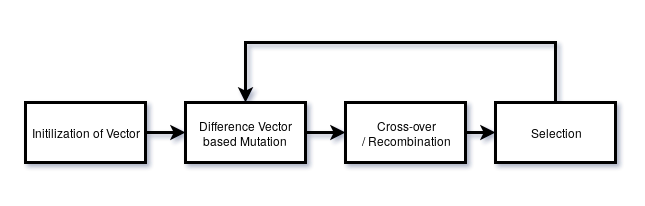
\includegraphics[scale=0.25]{figures/DE_stages.png}
    \caption{Stages in DE}
    \label{DE_stages}
    \end{center}
\end{figure}

\begin{itemize}

\item Initialization : \(x_{n}^{d}=L^{d}+\operatorname{rand}(0,1)\left(U^{d}-L^{d}\right)\)
\item Mutation : \(\mathbf{v}_{n}=\mathbf{x}_{r_{1}}+F\left(\mathbf{x}_{r_{2}}-\mathbf{x}_{r_{3}}\right)\)
\item Crossover : \(u_{n}^{d}=\left\{\begin{array}{ll}{v_{n}^{d}} & {\text { if rand }(0,1) \leq C R \text { or } r_{n}=d} \\ {x_{n}^{d}} & {\text { otherwise }}\end{array}\right.\)
\item Selection : \(\mathbf{x}_{n,g+1}=\left\{\begin{array}{ll}{\mathbf{u}_{n}} & {\text { if } f\left(\mathbf{u}_{n}\right) \leq f\left(\mathbf{x}_{n}\right)} \\ {\mathbf{x}_{n}} & {\text { otherwise }}\end{array}\right.\)
\item Stopping condition : Number of function evaluation.
\end{itemize}
}
\parbox{0.31\linewidth}{
\begin{figure}
    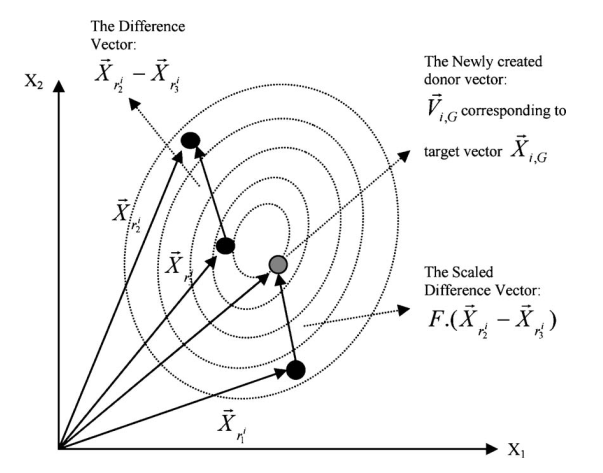
\includegraphics[scale= 0.18]{figures/Mutation.png}
    \caption{Mutation stage \cite{storn}}
    \label{Mutation}
    
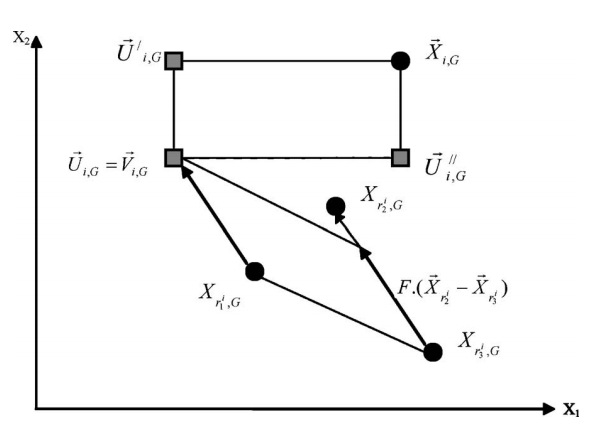
\includegraphics[scale = 0.18]{figures/crossover.png}
    \caption{Different possible trial vector formed due to Uniform/Binomial crossover between mutant vector and target vector in 2-D design space\cite{storn}.}
    \label{crossover}

\end{figure}
}
Two ways to implement the constraints:
\begin{itemize}
\item Penalty approach.
\item Using feasibility rules as mentioned by Deb and Saha\cite{Deb}.
\end{itemize}

\underline{Feasibility rules}:
\begin{itemize}
\item If both locations
are feasible, the one with the best fitness value wins.
\item If a single location is feasible, then
select the same.
\item Otherwise, select the location with the least constraint violations.
\end{itemize}
Mathematically,
\begin{equation}
\mathbf{x}_{a} \prec \mathbf{x}_{b}
\Leftrightarrow\left\{
\begin{array}{ll}
{f\left(\mathbf{x}_{b}\right)<f\left(\mathbf{x}_{a}\right)} & {\text { and } \quad \phi\left(\mathbf{x}_{a}\right), \phi\left(\mathbf{x}_{b}\right)=0} \\
{\phi\left(\mathbf{x}_{b}\right)=0} & {\text { and } \quad \phi\left(\mathbf{x}_{a}\right)>0} \\
{\phi\left(\mathbf{x}_{b}\right)<\phi\left(\mathbf{x}_{a}\right)} & {\text { and } \quad \phi\left(\mathbf{x}_{a}\right), \phi\left(\mathbf{x}_{b}\right)>0}
\end{array}\right.
\label{feas}
\end{equation}

where $\phi$ is the constraint violation given by:
\begin{equation}
\phi (\mathbf{x})=\sum_{i=1}^{p} \max \left[0, g_{i}(\mathbf{x})\right]+\sum_{j=1}^{q}\left|h_{j}(\mathbf{x})\right|
\end{equation}

where, $g_i(\textbf{x})$ represents the $i$-th inequality constraint value, and $h_j(\textbf{x})$ represents the $j$-th equality constraint value. 

At selection stage:

\begin{equation}
\mathbf{x}_{n}(t+1)=\left\{\begin{array}{ll}{\mathbf{u}_{n}} & {\text { if } \mathbf{x}_{n}(t) \prec \mathbf{u}_{n}} \\ {\mathbf{x}_{n}(t)} & {\text { otherwise }}\end{array}\right.
\label{selection_constraint}
\end{equation}
\newpage
\underline{Decomposition of algorithm:}
\begin{figure}
\parbox{0.47\linewidth}{
    
    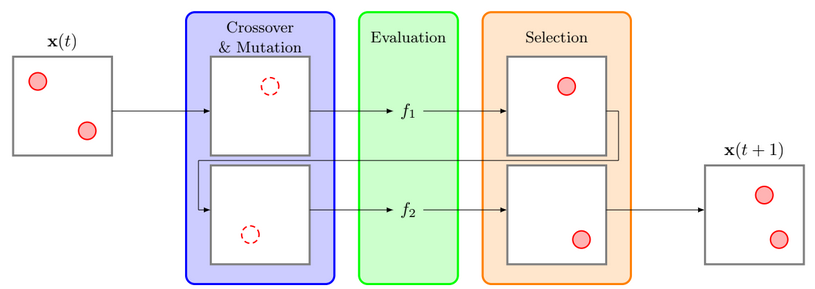
\includegraphics[scale = 0.16]{figures/sequential_form_DE.png}
    \caption{Sequential decomposition of algorithm\cite{Poole2}.}
    \label{sequential_form_algo}
    }
    \parbox{0.47\linewidth}{
    
    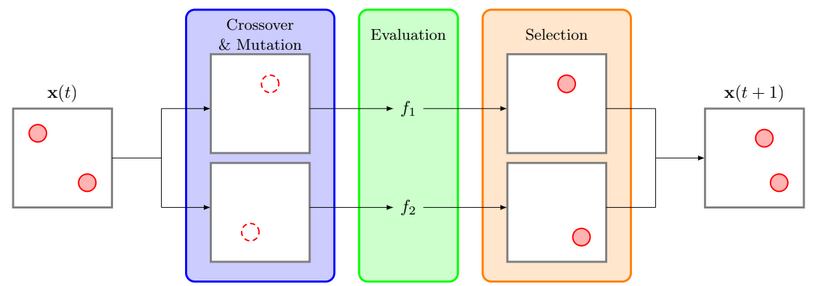
\includegraphics[scale = 0.16]{figures/parallel_form_DE.png}
    \caption{Parallel decomposition of algorithm\cite{Poole2}.}
    \label{parallel_form_algo}
    }
\end{figure}
\begin{itemize}
\item Sequential decomposition involves following all the DE steps for individual, then proceeding to next individual.
\item In parallel decomposition, for all individuals in a population all DE steps are carried in parallel.
\end{itemize}
 \vspace{1mm}
\underline{Niching algorithms:} These algorithms are able to capture multimodal optima in given design space. 
\begin{itemize}
    \item FDE:Feasible DE.
    \item FCDE:Feasible crowding DE.
    \item FSDE:Feasible species-based DE.
    \item FNRAND1: Feasible DE using nrand1 mutation, so on.
\end{itemize}
\newpage
\underline{FNRAND1 algorithm:}
\begin{itemize}
\item Although above mentioned algorithm are implemented on test cases, only the fNRAND1 algorithm is shown here.
\end{itemize}

\begin{figure}
    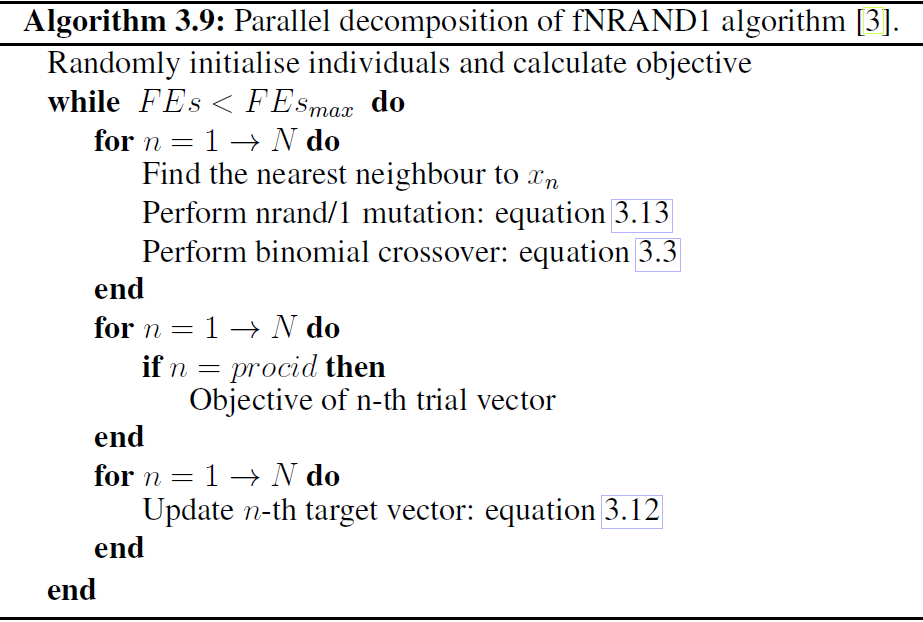
\includegraphics[scale = 0.192]{figures/parallel_decompo_fNRAND1.png}
    \caption{Parallel decomposition fINRAND1}
    \label{fINRAND1_algorithm}
\end{figure}
\underline{Test case:} Sphere function
\begin{equation}
f(\mathbf{x})=\sum_{i=1}^{d} x_{i}^{2}
\label{sphere function}
\end{equation}
\newpage
\underline{Outcome of FNRAND1 algorithm:}
\begin{itemize}
\item Optimization of 2D problem with design space between +3 and -3.
\item Figure (a) represents the initial population.
\item Elliptical constraint is used.

\end{itemize}

\begin{figure}
    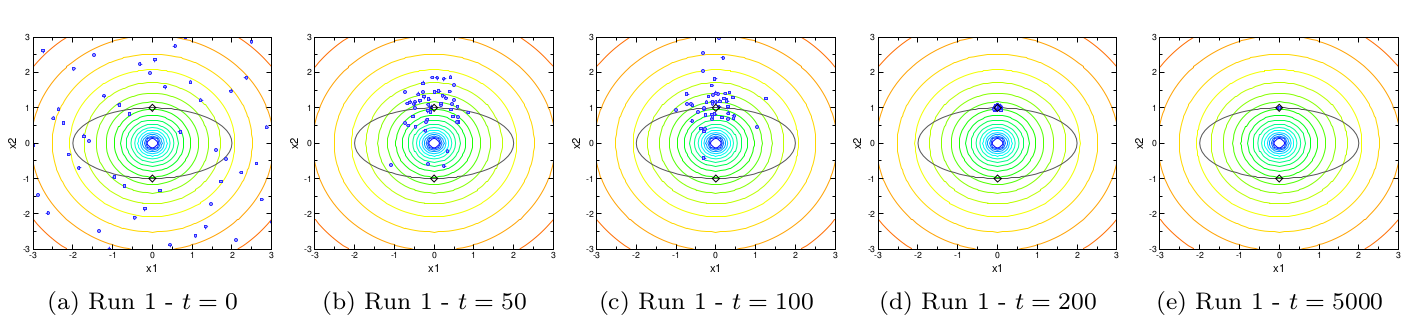
\includegraphics[width = 98mm,height= 30mm]{figures/iteration_convergence.png} 
    \caption{converging to optimal points}
    \label{convergence}
    \end{figure}
    
\begin{itemize}
\item Subsequent figure represents the progress of algorithm with generations.
\item Figure (e) represents the optimized values (two optima) at (+1, +1), and (+1,  -1).
\item This confirms that fNRAND1 is able to capture multiple optima in given design space.
\end{itemize}
\end{frame}
